\documentclass[tikz,border=2pt]{standalone}
\usepackage{tikz}

\begin{document}
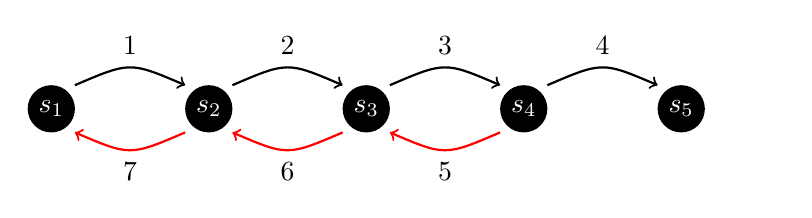
\begin{tikzpicture}[scale=2.0]

\def\r{0.15};
\foreach \x in {1,...,5}{
	\fill[fill=black] (\x, 0) circle [radius=\r];
	\node[white] at (\x, 0) {$s_{\x}$};
}
\fill[fill=white] (5.5, 0) circle [radius=\r];
\foreach \x in {1,...,4}{
	\draw [black, thick, ->] (\x+\r, \r) .. controls (\x+0.5, 0.3) .. (\x+1-\r, \r);
	\node at (\x+0.5, 0.4) {\x};
	}
\foreach[evaluate={\y=int(8-\x)}] \x in {1,...,3}{
	\draw [red, thick, <-] (\x+\r, -\r) .. controls (\x+0.5, -0.3) .. (\x+1-\r, -\r);
	\node at (\x+0.5, -0.4) {\y};
	}

\end{tikzpicture}
\end{document}
